\documentclass[12pt]{article}
\usepackage[paper=letterpaper,margin=2cm]{geometry}
\usepackage{amsmath}
\usepackage{amssymb}
\usepackage{amsfonts}
\usepackage{newtxtext, newtxmath}
\usepackage{enumitem}
\usepackage{titling}
\usepackage[colorlinks=true]{hyperref}
\usepackage{graphicx}
\usepackage{float}
\usepackage{listings}
\usepackage{xcolor}
\usepackage{color}
\definecolor{dkgreen}{rgb}{0,0.6,0}
\definecolor{gray}{rgb}{0.5,0.5,0.5}
\definecolor{mauve}{rgb}{0.58,0,0.82}
\lstset{ %
        language=Java,                
  basicstyle=\footnotesize,     
  numbers=left,               
  numberstyle=\tiny\color{gray},
  stepnumber=1,                                       
  numbersep=5pt,                 
  backgroundcolor=\color{white},  
  showspaces=false,             
  showstringspaces=false,         
  showtabs=false,                 
  frame=single,                   
  rulecolor=\color{black},       
  tabsize=4,                   
  captionpos=b,        
  breaklines=true,             
  breakatwhitespace=false,       
  title=\lstname,                                                  
  keywordstyle=\color{blue},          
  commentstyle=\color{dkgreen},    
  stringstyle=\color{mauve},       
  escapeinside={\%*}{*},        
  morekeywords={*,...}
} 

\setlength{\droptitle}{-6em}

% Enter the specific assignment number and topic of that assignment below, and replace "Your Name" with your actual name.
\title{Assignment 2: Comp 6771 Image Processing}
\author{Yunqi Xu 40130514}
\date{\today}



\begin{document}
% \maketitle

\begin{titlepage}
  \rule{\textwidth}{1pt}   % The top horizontal rule
    \vspace{0.2\textheight}  % Whitespace between top horizontal rule and title

    %------------------------------------------------------------
    %    Title
    %------------------------------------------------------------

    {\Huge COMP 6771 Image Processing: Assignment 2}

    \vspace{0.025\textheight}   % Whitespace between the title and short horizontal rule

    \rule{0.83\textwidth}{0.4pt}  % The short horizontal rule under title

    \vspace{0.1\textheight}  % Whitespace between the short horizontal rule and author

    %------------------------------------------------------------
    %    Author
    %------------------------------------------------------------

    {\Large Student name: \textsc{Yunqi Xu}}
    \vfill
    {\Large Student id: 40130514}
    \vfill  % Whitespace between author and date

    {\large \today}
    \vspace{0.1\textheight}  % Whitespace between date and bottom horizontal rule

    %------------------------------------------------------------
    %    Bottom rules
    %------------------------------------------------------------

    \rule{\textwidth}{1pt}  % The bottom horizontal rule
\end{titlepage}

\begin{enumerate}[leftmargin=\labelsep]
% \vspace*{40em}
\item Question 1
    \begin{enumerate}
        \item Based on the question, the mask is:
        \begin{equation}
            g(x, y) = \frac{1}{4}[f(x, y-1) + f(x, y+1) +f(x-1, y) +f(x+1, y)]  
            \label{q1_eq1}    
        \end{equation}
        Also, 
        \begin{equation}
            f(x - x_{0}, y - y_{0}) = F(u, v)e^{-j2 \pi (ux_{0}/M + vy_{0}/N)}
            \label{q1_eq2}
        \end{equation}

        Based on the Eq.~\ref{q1_eq2}, the Eq.~\ref{q1_eq1} can be calculated like:
        \begin{equation}
        \begin{aligned}
        f(x, y-1)
        &= f(x - 0, y -(1))\\
        &= f(u, v)e^-j2\pi(u(0)/M + v(1)/N)\\
        &= F(u, v)e^{-j2\pi v/N}
        \label{q1_eq3}
        \end{aligned}
        \end{equation}
        
        \begin{equation}
            \begin{aligned}
                f(x, y+1) 
                &= f(x-0, y-(-1))\\
                &= F(u, v)e^{-j2\pi (u(0)/M + v(-1)/N)}\\
                &= F(u, v)e^{j2\pi u/M}
            \label{q1_eq3}
            \end{aligned}
        \end{equation}

        \begin{equation}
            \begin{aligned}
                f(x -1, y) 
                &= f(x-(1), y-0)\\
                &= F(u, v)e^{-j2\pi(u(1)/M + v(0)/N)}\\
                &= F(u, v)e^{-j2\pi u/M}
            \label{q1_eq4}
            \end{aligned}
        \end{equation}

        \begin{equation}
            \begin{aligned}
                f(x -1, y) 
                &= f(x-(1), y-0)\\
                &= F(u, v)e^{-j2\pi(u(1)/M + v(0)/N)}\\
                &= F(u, v)e^{-j2\pi u/M}
            \label{q1_eq4}
            \end{aligned}
        \end{equation}


        \begin{equation}
            \begin{aligned}
                f(x +1, y) 
                &= f(x-(-1), y-0)\\
                &= F(u, v)e^{-j2\pi(u(-1)/M + v(0)/N)}\\
                &= F(u, v)e^{-j2\pi u/M}
            \label{q1_eq5}
            \end{aligned}
        \end{equation}
        
        So, based on the Eq.~\ref{q1_eq2} ~\ref{q1_eq3} ~\ref{q1_eq4} ~\ref{q1_eq5}, 

        \begin{equation}
            G(u, v) = \frac{1}{4} F(u, v) [e^{-j2\pi v/N} + e^{j2\pi v/N} + e^{j2\pi u/M} + e^{j2\pi u/M}]
        \end{equation}

        \begin{equation}
            H(u, v) = \frac{1}{4} [e^{-j2\pi v/N} + e^{j2\pi v/N} + e^{j2\pi u/M} + e^{j2\pi u/M}]
        \end{equation}

        Based on the Euler's Formula, $$\cos \theta = \frac{1}{2}(e^{i \theta} + e^{-i \theta})$$,

        \begin{equation}
            \begin{aligned}
                H(i, v)
                &= \frac{1/4}F(u, v)[2\cos(\frac{2 \pi v}{N} + 2\cos(\frac{2\pi u}{M}))]\\
                &= \frac{1}{2}F(u, v)[\cos(\frac{2 \pi v}{N} + \cos(\frac{2\pi u}{M}))]
            \end{aligned}
        \end{equation}

    \vspace*{1em}
    \end{enumerate}

\item Question 2

\begin{enumerate}
    \item  If an equation is linear, which means that:
    \begin{equation}
        O(af_{1}(x, y) + bf_{2}(x, y)) = aO(f_{1}(x, y)) + bO(f_{2}(x, y))
        \label{q2_eq1}
    \end{equation}
    In Eq.~\ref{q2_eq1}, the $O()$ is an operator.
    So in this queation:
    \begin{equation}
        \begin{aligned}
        O(af_{1}(x, y) + bf_{2}(x, y))
        &= \int_{-\infty}^{\infty}\int_{-\infty}^{\infty}(af_1(x, y) + bf_2(x, y))\delta(x\cos\theta + y\sin\theta - \rho)dxdy\\
        &= a\int_{-\infty}^{\infty}\int_{-\infty}^{\infty}f_1(x, y)\delta(x\cos\theta + y\sin\theta - \rho)dxdy + \\
        & b\int_{-\infty}^{\infty}\int_{-\infty}^{\infty}f_2(x, y)\delta(x\cos\theta + y\sin\theta - \rho)dxdy\\
        &= aO(f1(x, y)) + bO(f2(x, y))
        % \label(q2_eq2)
        \end{aligned}
    \end{equation}
    So it is linear operator.

    \item Based on the priciple of Integral by substitution:
    \begin{equation}
     \begin{aligned}
        u = x - x_0\\
        v = y - y_0
        \end{aligned}
    \end{equation}

    \begin{equation}
        \begin{aligned}
            du = dx \\
            dv = dy
        \end{aligned}
    \end{equation}

    \begin{equation}
        \begin{aligned}
                f(\rho, \theta)
                &= \int_{-\infty}^{\infty}\int_{-\infty}^{\infty}f(x - x_0, y - y_0) \delta(x\cos\theta + y\sin\theta - \rho)dxdy\\
                &= \int_{-\infty}^{\infty}\int_{-\infty}^{\infty}f(u, v)\delta[(u + x_0)\cos\theta + (v + y_0)\sin\theta - \rho)dudv\\
                &= \int_{-\infty}^{\infty}\int_{-\infty}^{\infty}f(u, v)\delta(u\cos\theta + x_0\cos\theta + v\sin\theta + y_0\sin\theta - \rho)dudv\\
                &= \int_{-\infty}^{\infty}\int_{-\infty}^{\infty}f(u, v)\delta(u\cos\theta + v\sin\theta - (\rho - x_0\cos\theta - y_0\sin\theta))dudv\\
                &= g(\rho - x_0\cos\theta - y_0\sin\theta, \theta)
        \end{aligned}
    \end{equation}    

\end{enumerate}

\item Programming Question 1 
\begin{enumerate}
\item The code is shown blow.
\begin{lstlisting}
    %read image
    img_house = imread("house.tif");
    img_jet = imread("jet.tiff");
    img_house = img_house(:, :, 1);
    img_jet = img_jet(:, :, 1);
    
    
    % Fourier Transformer
    img_house_f = fft2(double(img_house));
    img_jet_f = fft2(double(img_jet));
    
    %calculate the magnitude and phase of house
    img_house_m = abs(img_house_f);
    img_house_ph = angle(img_house_f);
    
    %calculate the magnitude and phase of jet
    img_jet_m = abs(img_jet_f);
    img_jet_ph = angle(img_jet_f); 
    
    %reconstruct images
    image_a=img_house_m.*cos(img_jet_ph)+img_house_m.*sin(img_jet_ph).*1i;
    image_b=img_jet_m.*cos(img_house_ph)+img_jet_m.*sin(img_house_ph).*1i;
    image_a=abs(ifft2(image_a));
    image_b=abs(ifft2(image_b));
    image_a=uint8(image_a);
    image_b=uint8(image_b);
    
    
    % plot images
    subplot(2,2,1);imshow(img_house);title('House');
    subplot(2,2,2);imshow(img_jet);title('Jet');
    subplot(2,2,3);imshow(image_a);title('Magenitude of house with phase of Jet');
    subplot(2,2,4);imshow(image_b);title('Magnitude of Jet with phase of House');
\end{lstlisting}

The images are shown below:
\begin{figure}[H]
    \centering
    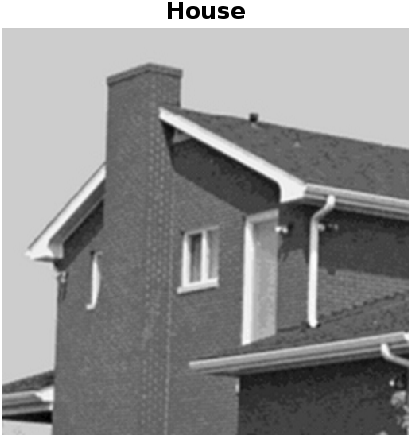
\includegraphics[]{Figure/House.png}
    \caption{Input House}
    \label{Q3_1}
\end{figure}

\begin{figure}[H]
    \centering
    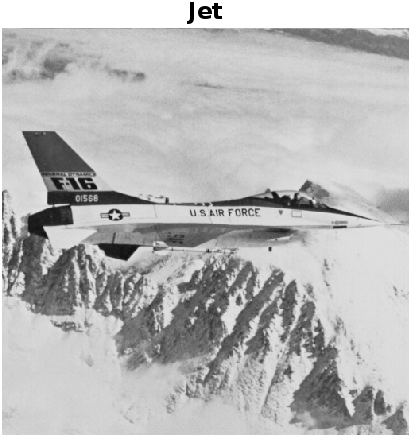
\includegraphics[]{Figure/Jet.png}
    \caption{Input Jet}
    \label{Q3_2}
\end{figure}

\begin{figure}[H]
    \centering
    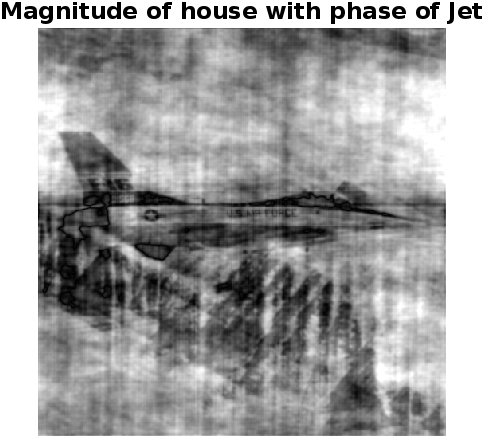
\includegraphics[]{Figure/Magnitude of house with phase of Jet.png}
    \caption{Magnitude of house + phase of Jet}
    \label{Q3_3}
\end{figure}

\begin{figure}[H]
    \centering
    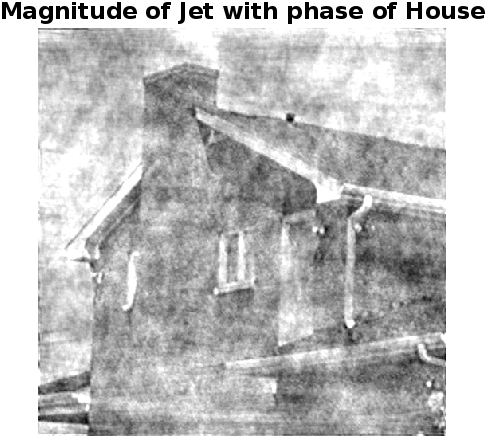
\includegraphics[]{Figure/Magnitude of Jet with phase of House.png}
    \caption{Magnitude of Jet + phase of House}
    \label{Q3_4}
\end{figure}

Suppoer the Fig.~\ref{Q3_1} is $I_A$, so the Fig.~\ref{Q3_4} have a better result to reconstruct the Fig.~\ref{Q3_1} compared with Fig.~\ref{Q3_3}. On the other hand, the Fig.~\ref{Q3_3} reconstruct will for Fig.~\ref{Q3_2}. Because the phase of the Fourier of an image keep more information compared with magnitude of the image. So it is clearly to find that in Fig.~\ref{q3_3} the Jet keep more information, and in Fig.~\ref{q3_4} there are more information present the house.

\end{enumerate}


\item Programming q2
\begin{enumerate}
    \iten the code is shown below
        
\end{enumerate}

\end{enumerate}

\end{document}
